Because no public datasets of SQL antipatterns in jOOQ currently exist, this chapter details the methodology used to establish a ground truth. We describe the process of mining and filtering publicly available projects from GitHub, followed by the strategies used for sample generation, manual annotation, and splitting the data into training, validation, and test sets.

\section{Repository Mining}\label{sec:mining}

We started by mining software repositories for projects, which we would later use for evaluation and analysis purposes. We wanted to collect as many projects as possible within reason, matching the following criteria:
\begin{itemize}
    \item the project contains Java code that uses jOOQ for database access,
    \item the project stores jOOQ-generated classes as part of the source code, rather than treating them as derived artefacts, which are not put under version control \nobreakcite{jooq2025code}.
\end{itemize}

The latter criterion was required to exclude projects that would otherwise have needed to be compiled in order to detect database design antipatterns. Due to the wide variety of Java versions, build tools, and configurations used in the projects, this would have required a large amount of manual effort on a project-by-project basis, which we opted against. For a considerable number of projects, this would have also been impossible for reasons such as private or otherwise unavailable dependencies, as well as jOOQ code generator configurations only capable of working on the original developer's machine.

To achieve this goal, we used the GitHub code search API \nobreakcite{githubSearchApi}, to search for projects that use jOOQ. The GitHub search API has a hard limit of \num{1000} results for each search term \nobreakcite{githubSearchApi}, which required us to minimise the number of duplicated results for each search term. For example, this meant that we could not search for import statements for jOOQ classes within Java files, since a few large projects could saturate the result list.

To find the largest number of unique projects possible, we limited our search to the manifest files of projects, looking for statements, which declare a dependency on jOOQ for the project. We limited the search to the manifest file formats of the two most popular build tools for Java \nobreakcite{stackOverflowSurvey}: Maven \nobreakcite{maven2026homepage} (e.g., \texttt{pom.xml}) and Gradle \nobreakcite{gradle2026homepage} (e.g., \texttt{build.gradle} and \texttt{build.gradle.kts}). We designed the search terms to be as specific as possible to keep the number of results below \num{1000} when possible. For some search terms, the number of matching results exceeded the limit of \num{1000}. In these cases, we retrieved the \num{1000} results that had been indexed most recently by GitHub’s search infrastructure. The list of search terms used in the GitHub search API is provided in Appendix~\ref{chapter:appendix-github-search-terms}.

By performing the search on 10 January 2026, we identified \textbf{\num{3829}} projects that declared a dependency on jOOQ. We further filtered the gathered repositories by checking that the previously set criteria are met by making sure that the repositories contain jOOQ-generated classes as well as other Java files with references to jOOQ classes.

After excluding projects that did not store generated classes as part of their source code, we were left with \textbf{\num{802}} projects. Although not relevant to our research, an interesting observation can be made here: while both storing generated classes as part of the source code and treating them as derived artefacts are valid approaches with their merits and drawbacks \nobreakcite{jooq2025code}, only \qty{21}{\percent} of projects store them as part of the source code. We suspect that this is largely because the jOOQ code generator treats them as derived artefacts by default.

After excluding projects that did not contain any non-generated Java classes referencing jOOQ, we were left with \textbf{\num{645}} projects. The projects omitted by this step were mostly projects written in other programming languages running on the Java Virtual Machine (JVM), such as Kotlin and Scala.

Finally, we performed manual, LLM-assisted cleaning, with the aim of removing duplicate projects, which could later cause cross-contamination between training, validation, and test sets. We performed the analysis of duplicates with the Google Gemini 3 Pro Preview \nobreakcite{gemini3ProPreview} model from its web interface. We provided the LLM with the file trees of the \num{645} remaining projects, prompting it to find potential clones and forks. We selected the model for its large context window, which was required to process the large collection of file trees, combined with its high reasoning capabilities. Although the LLM did a remarkable job with the task, we manually reviewed the findings before any omissions.

For various reasons documented in Appendix~\ref{chapter:appendix-omitted-projects}, we omitted \num{42} projects. Most importantly, we found and removed \num{24} copies of a repository containing numerous Java- and Spring-related tutorials created by Baeldung \nobreakcite{baeldungHomepage}. While we also found a similarly sized cluster of projects created as part of a Java course by the Tinkoff bank in Russia, all of which had a similar structure and database schema, we decided to keep these projects, since each of them was created by a different author and had a distinct implementation and contained varying antipatterns. After the clean-up, we were left with \textbf{603} projects.

Later in the research process, preparing for the large-scale project analysis (Chapter~\ref{chapter:projectAnalysis}), we discovered another large duplicated project, which would have skewed our analysis results. Hence, we later omitted that project from the analysis dataset, leaving us with \textbf{602} projects. The stages of mining and filtering projects are visualised in Figure~\ref{fig:dataFunnel}.

\begin{figure}[h]
    \centering
    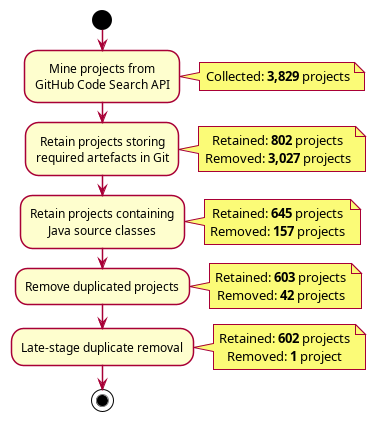
\includegraphics[width=200pt]{figures/data_funnel_diagram.png}
    \caption{Project mining and filtering stages.}
    \label{fig:dataFunnel}
\end{figure}

\subsection{Considered Alternatives}\label{sec:miningAlternatives}

Our method of mining repositories by using the GitHub code search API has the downside of being incomprehensive, meaning that it misses a portion of the projects available on GitHub for any of the following reasons:

\begin{itemize}
    \item the project does not use a build tool,
    \item the project uses a build tool that is not Maven or Gradle,
    \item the project is \textbf{only} found by search terms, which return over \num{1000} results, and the project is omitted due to not being indexed recently.
\end{itemize}

Although the portion of missed projects is low (no other Java build tool is anywhere near the popularity of Maven and Gradle \nobreakcite{stackOverflowSurvey}, and the more specific search terms should have caught all projects missed by the broader ones), it is a valid reason to mention alternative solutions we considered for mining Java repositories, and why we opted against using them.

\nobreaktextcite[p. 209]{allamanis2013mining} presented a curated corpus of \num{14807} open-source Java projects sourced from GitHub. As their work was published in 2013, it is outdated by 2026: a large part of the projects in the corpus has been deleted (as reported by \nobreaktextcite[p. 552]{goeminne2015towards} in 2015), new projects are missing, and the remaining projects could be using deprecated jOOQ APIs. Furthermore, their original corpus only contained ten projects using jOOQ \nobreakcite[Fig. 1]{goeminne2015towards}. 

We considered creating an up-to-date version of the corpus by repeating the work of Allamanis and Sutton, processing GitHub's event stream, provided by GH Archive \nobreakcite{ghArchive2026homepage}. However, the dataset has grown rapidly since 2013, and combined with the suboptimal structure of the GH Archive dataset \nobreakcite{ghArchiveLinkedIn}, it would have required us to commit an unreasonable amount of resources, given the preliminary nature of this research step. 

\nobreaktextcite[p. 58]{sharma2018smelly} employed RepoReaper \nobreakcite{DBLP:journals/ese/MunaiahKCN17} to select open-source repositories for their study, finding \num{2568} high-quality projects in various programming languages, which contained SQL statements. However, RepoReaper used GHTorrent \nobreakcite{DBLP:conf/msr/Gousios13} to obtain metadata about GitHub repositories \nobreakcite[p. 3223]{DBLP:journals/ese/MunaiahKCN17}, and GHTorrent has not been updated since early 2021 \nobreakcite{ghTorrentReddit}. Therefore, any set of projects produced based on GHTorrent would suffer from similar issues as the original corpus from Allamanis and Sutton.

Consequently, we found that our approach using the GitHub code search API is the best option available to us without committing unreasonable effort or resources.

\section{Establishment of Ground Truth}\label{sec:groundTruth}

To evaluate the detection performance of the prompting strategies and our later developed tool, we required a source of ground truth. As SQL antipatterns in jOOQ represent an unexplored area, to the best of our knowledge, no publicly available datasets of SQL antipatterns in jOOQ currently exist. Furthermore, the scientific literature provides no examples of how SQL antipatterns may occur in jOOQ, and such examples are also scarce elsewhere. For example, a remark in the jOOQ manual \nobreakcite{jooq2025select} shows that the “Implicit Columns” antipattern \nobreakcite[Ch. 19]{karwin2023sql} can occur in jOOQ in unexpected ways. Therefore, examples of antipatterns in plain SQL alone are insufficient for detecting SQL antipatterns in jOOQ.

To establish the ground truth, we manually annotated a subset of the projects gathered in Section~\ref{sec:mining}.

\subsection{Sample Generation}\label{sec:sampleGeneration}

As the projects are of varying size, we wanted the subset to be representative of the complete set of projects regarding size distribution, avoiding bias towards small or large projects. Figure~\ref{fig:distribution} displays the distribution of the number of relevant database access files per project across our dataset of \num{603} projects (still including the duplicated project that was filtered out at a later stage). We consider a Java source file to be a relevant database access file if both of the following conditions are met:

\begin{itemize}
  \item it is a jOOQ-generated file or contains references to jOOQ or a generated file,
  \item it is not considered “irrelevant” by a manually compiled path list.
\end{itemize}

 The path list consisted of jOOQ-generated files that were not useful for antipattern detection (e.g., records and POJOs), and files generated based on database entities not part of the project, such as system schemas of databases and tables managed by database extensions.

\begin{figure}[h]
    \centering
    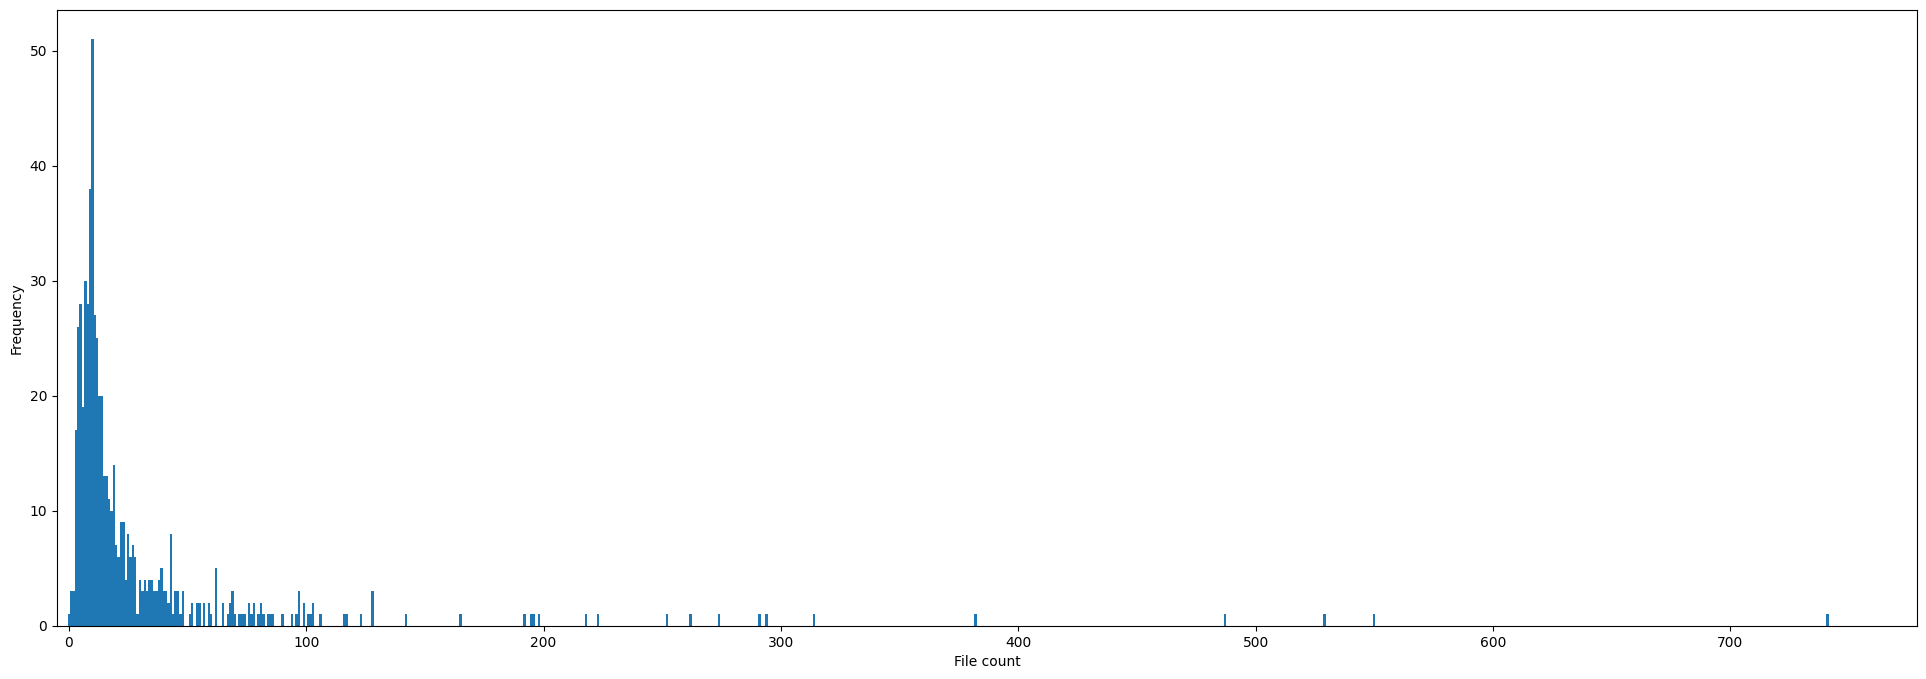
\includegraphics[width=\textwidth]{figures/distribution_of_files.png}
    \caption{Distribution of relevant database access files per project.}
    \label{fig:distribution}
\end{figure}

It should be noted that at this stage of the study, the list of “irrelevant” files was inconclusive and had some omissions, which we only discovered later. In Figure~\ref{fig:distributionCorrected}, we show the file distribution of 602 projects, omitting the later-discovered duplicated project, as well as using the final file list from a later stage of the study. It can be seen that, while the graph shifts slightly, the overall distribution remains similar.

\begin{figure}[h]
    \centering
    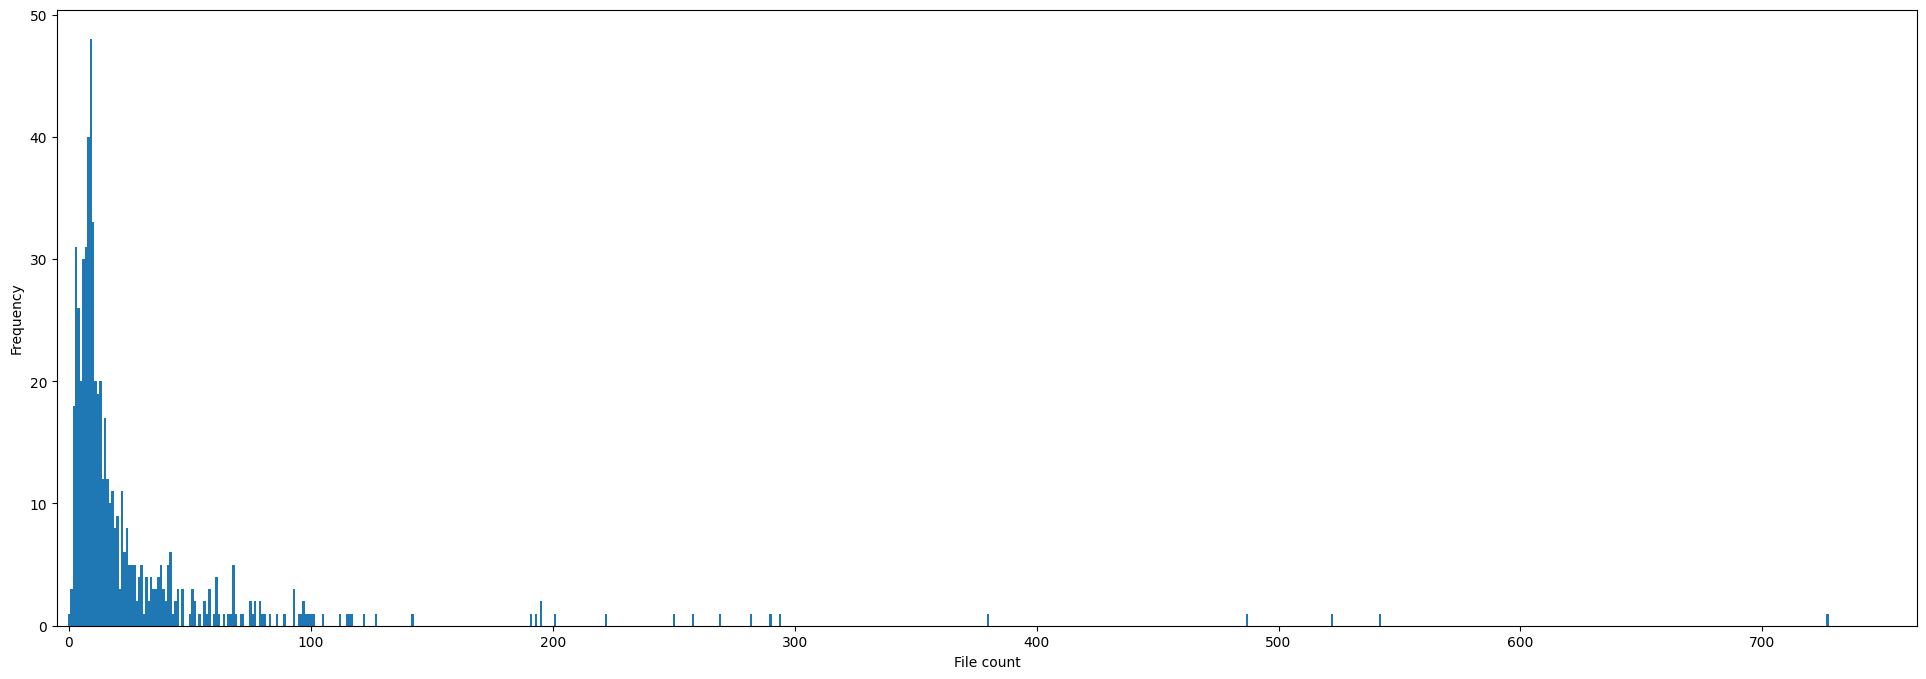
\includegraphics[width=\textwidth]{figures/distribution_of_files_corrected.png}
    \caption{Distribution of relevant database access files per project (corrected).}
    \label{fig:distributionCorrected}
\end{figure}

As illustrated in the figures, the project distribution is positively skewed, with most projects clustered near zero (the “head”) and a small number of substantially larger projects forming the “long tail”. To ensure that small, medium, and large projects are adequately represented, we employed a stratified random sampling approach, selecting an equal percentage of projects from each group. Our initial plan was to select \qty{5}{\percent} of the projects, but we later increased it to \textbf{\qty{10}{\percent}} due to an insufficient number of antipattern samples.

We divided the projects into size groups using the Head-Tail Breaks method. Given the set of projects as \(S\) and an individual project \(x\), we calculated the two breakpoints, \(\mu_1\) and \(\mu_2\), which represent the upper file limits for small and medium projects:
\begin{equation}
\mu_1 = \frac{1}{|S|} \sum_{x \in S} x
\end{equation}
\begin{equation}
S_{head} = \{ x \in S \mid x > \mu_1 \}
\end{equation}
\begin{equation}
\mu_2 = \frac{1}{|S_{head}|} \sum_{x \in S_{head}} x
\end{equation}

Based on these breakpoints, we classified the projects as:
\begin{equation}
\text{Class} = \begin{cases} 
      \text{Small} & x \le \mu_1 \\
      \text{Medium} & \mu_1 < x \le \mu_2 \\
      \text{Large} & x > \mu_2 
   \end{cases}
\end{equation}

We found the breakpoints to be \textbf{\num{31}} and \textbf{\num{94}}. Using these breakpoints, we classified \num{467} projects as small, \num{100} projects as medium, and \num{36} projects as large. Using the distribution from Figure~\ref{fig:distributionCorrected}, the numbers would have been slightly altered: the breakpoints would have been \num{29} and \num{91}, and the class sizes would have been \num{468}, \num{98}, and \num{36}.

Using the former classifications, we sampled \qty{10}{\percent} of projects from each size class, resulting in \num{47} small, ten medium, and four large projects. In total, the sample of projects selected for annotation contained \textbf{61} projects. We used the fixed seed \num{123456} for the pseudo-random number generator used for sampling, which ensures that the sampling process is consistent and reproducible.

\subsection{Antipattern Selection}\label{sec:antipatternSelection}

We limited the annotated antipatterns to the ones defined by \nobreaktextcite{karwin2023sql}. Although we attempted to maximise the number of antipatterns included in our analysis and to interpret them as closely as possible to Karwin’s definitions, we made several notable exclusions and interpretational deviations.

We excluded the “Index Shotgun” antipattern from our analysis. \nobreaktextcite[pp. 147--152]{karwin2023sql} recommends using the MENTOR (Measure, Explain, Nominate, Test, Optimize, and Rebuild) framework to choose optimal indexes. The framework involves measuring the runtime performance of SQL queries—a step that cannot be replaced by static analysis. Although other practitioners, such as \nobreaktextcite[pp. vi-vii]{Winand2012}, recommend creating optimal indexes during the development process, which could be aided by static analysis, choosing optimal indexes for a table can be a complex process with many trade-offs and deserves more dedicated research to be addressed appropriately.

We restricted our definition of the “Fear of the Unknown” antipattern to only include occurrences that are caused by flawed database design, as well as query conditions, which do not contain values passed in from Java code. As the type system of Java is not null-safe, Java code can contain many potential nullability errors, but detecting them would have caused a large additional annotation burden. Furthermore, specialised tools (e.g., NullAway \nobreakcite{DBLP:conf/sigsoft/BanerjeeCS19}) exist for detecting nullability errors in Java more efficiently and accurately.

\nobreaktextcite[p. 151]{nagy2017static} excluded the “Spaghetti Query” antipattern from their analysis, arguing that there is no objective definition to determine whether a query is a spaghetti query or not. They considered metrics, such as the length of a query in lines or characters, and counts of joins and subqueries, but found them too subjective.

Such metrics also do not tell the full picture, since one large query can often outperform multiple small queries due to optimisations in the database engine, and two queries with a similar length, involving the same number of tables, can differ vastly in their readability and performance. For example, \nobreaktextcite{Dombrovskaya2024} describe several techniques for factoring large queries to improve their performance, readability, or reusability. Furthermore, the use of jOOQ DSL makes it possible to factor the source code of queries using object-oriented principles, further aiding with readability and reusability. For these reasons, we excluded the “Spaghetti Query” antipattern from our analysis.

We extended our definition of “Implicit Columns” to also include other types of blind projections, which select every column from a table, such as API methods, which fetch generated records from the database \nobreakcite{jooq2025select}. Such blind projections are considered a bad practice according to the jOOQ documentation, having similar negative effects to the cases described by Karwin \nobreakcite{jooq2025select}.

We also excluded “Pseudokey Neat-Freak” and “Diplomatic Immunity” from our analysis, since they are rooted in organisational culture and cannot be detected from source code. Additionally, the use of jOOQ DSL largely mitigates the “Diplomatic Immunity” antipattern because SQL statements become first-class citizens of Java code.

Finally, we excluded the “See No Evil” antipattern due to difficulties in detecting it without performing runtime analysis. Unlike the Python examples provided by Karwin \nobreakcite[p. 270]{karwin2023sql}, Java projects using modern application frameworks do not usually perform fine-grained database exception handling for each database-related statement, but apply a retry mechanism at a transaction boundary, or use global exception handlers (e.g., in Spring \nobreakcite{spring2026exceptionHandler} and Micronaut \nobreakcite{micronaut2026exceptionHandler}), which could be implicitly installed by the framework. This makes accurate detection of the antipattern difficult for both human annotators and static analysis tools.

In total, we selected 19 antipatterns for annotation, including 8 logical design antipatterns, 3 physical design antipatterns, 5 query antipatterns, and 3 application development antipatterns. The list of included antipatterns by category is provided in Appendix~\ref{chapter:appendix-annotated-antipatterns}.

\subsection{Annotation Process}

Based on prior experience with jOOQ and SQL antipatterns, we manually assigned labels to antipattern occurrences found in the 61 sampled projects by carefully manually reviewing their source code. We tracked the labels in a LibreOffice spreadsheet, which we later converted into a comma-separated values (CSV) file. For each antipattern occurrence, we marked down the following information:
\begin{itemize}
    \item the type of antipattern,
    \item the project containing it,
    \item the path of the file containing it, relative to the root directory of the project,
    \item the start and end of the line span of the occurrence,
    \item a brief remark about the occurrence.
\end{itemize}

Due to the wide variety of Java versions, build tools, and local deployment methods used in the projects, along with occasional unavailable dependencies, we did not perform any runtime analysis on the projects.

As we studied a novel intersection between jOOQ and SQL antipatterns, not enough annotators sufficiently qualified in both domains were available to achieve a multi-annotator setup. Consequently, we employed a single-annotator setup, utilising the following means to maximise internal consistency.

\subsubsection*{Iterative Guideline Development}

During the annotation process, we created a codebook for the annotation process in the form of flowcharts available in Appendix~\ref{chapter:appendix-annotation-process-diagrams}.

During the annotation process, we followed the flowcharts for each antipattern, annotating their occurrences based on the visualised decision trees. When we spotted a variation of an antipattern or a non-antipattern edge case not yet covered by the corresponding decision tree, we adjusted the tree and re-reviewed previously, potentially incorrectly annotated files for consistency. This ensured that annotation decisions were made according to a consistent set of rules, rather than gut feeling.

\subsubsection*{Intra-Annotator Agreement}

After a 30-day washout period, we re-annotated a subset of the previously reviewed files to verify the stability of the annotation logic over time. We sampled \qty{10}{\percent} of the files containing at least one antipattern occurrence, and added an equivalent number of random files without antipattern occurrences to them. In total, we re-annotated \num{128} files using the same annotation guidelines. We used the fixed seed \num{123456} for the pseudo-random number generator used for sampling, which ensures that the sampling process is consistent and reproducible.

To measure the agreement between the two sets of annotations, we employed Cohen's Kappa ($\kappa$). However, traditional Kappa is designed for nominal classification and does not account for the spatial displacement inherent in a multi-occurrence localisation task. Consequently, we adapted the metric to determine whether the two sets of annotations contain the same antipattern occurrences based on an exact spatial match.

We define a line span \(S\) as the set of line indices within an inclusive range in a source code file.
\begin{equation}
S = \{i \in \mathbb{N} \mid start \le i \le end\}
\end{equation}

Given two annotators \(A\) and \(B\), and their annotated line spans \(S_A\) and \(S_B\), we consider the two line spans to match only if they cover the identical range of lines:
\begin{equation}
S_A = S_B
\end{equation}

After aligning the spans using this exact-matching gate, we constructed a \num{16} × \num{16} confusion matrix whose rows and columns represented the \num{15} distinct antipatterns annotated across the \num{128} files, together with the absence of an antipattern. The complete matrix is provided in Appendix~\ref{chapter:appendix-annotation-confusion-matrix}.

Given a set of \(k\) antipattern categories plus a “Background” category (\(k+1\) total classes), let \(n_{ij}\) denote the number of occurrences where Annotator A assigned class \(i\) and Annotator B assigned class \(j\). The total number of unique candidate occurrences is \(N = \sum_{i=1}^{k+1} \sum_{j=1}^{k+1} n_{ij}\).

The observed relative agreement (\(p_o\)) is defined as the proportion of occurrences where both annotators assigned the identical label to a spatially matching span:
\begin{equation}
p_o = \frac{1}{N} \sum_{i=1}^{k+1} n_{ii}
\end{equation}

The probability of random agreement (\(p_e\)) is calculated based on the marginal totals of the confusion matrix. Let \(n_{i \cdot}\) be the total number of times Annotator A used label \(i\), and \(n_{\cdot i}\) be the total number of times Annotator B used label \(i\). The expected agreement is defined as:
\begin{equation}
p_e = \frac{1}{N^2} \sum_{i=1}^{k+1} n_{i \cdot} n_{\cdot i}
\end{equation}

Where the marginal totals are derived as:
\begin{equation}
n_{i \cdot} = \sum_{j=1}^{k+1} n_{ij}, \quad n_{\cdot i} = \sum_{j=1}^{k+1} n_{ji}
\end{equation}

Finally, Cohen’s Kappa (\(\kappa\)) is computed to normalise the observed agreement against the possibility of chance:
\begin{equation}
\kappa = \frac{p_o - p_e}{1 - p_e}
\end{equation}

We found the Cohen's Kappa to be \textbf{\num{0.834}}. According to the standard scale by \nobreaktextcite{Landis77}, this represents an almost perfect agreement between the sets of annotations, demonstrating that the resulting dataset is internally consistent. Despite this, we acknowledge that the lack of an inter-annotator agreement check ultimately leaves the dataset vulnerable to the systematic blind spots of a single annotator.

\subsubsection*{Results}

In total, we annotated \textbf{\num{1562}} occurrences of 19 distinct SQL antipatterns within the \num{61} sampled projects. At least one occurrence of each antipattern was found in the sample, and every project in the sample contained at least one SQL antipattern occurrence. The most common antipatterns were “Implicit Columns”, which we found \num{795} occurrences of in 59 projects, and “ID Required” with \num{259} occurrences in \num{49} projects. In Table~\ref{tab:prevalenceInSample}, we show the prevalence of each SQL antipattern in the sampled projects.

\begin{longtable}[hp]{|p{3.5cm}|S[table-format=3, table-column-width=2cm]|S[table-format=2, table-column-width=2.5cm]|S[table-format=2.2, table-column-width=2.5cm]|S[table-format=2.2, table-column-width=3cm]|}
	\caption{Prevalence of SQL antipatterns in sampled projects.}
	\label{tab:prevalenceInSample}\\ \hline
	{\thead[l]{Antipattern}} & {\thead{Occurrence\\Count}} & {\thead{Containing\\Project Count}} & {\thead{Occurrences\\per Project}} & {\thead{Occurrences per\\Containing Project}}  \\
	\hline
	\endfirsthead
	\multicolumn{5}{l}
	{\tablename\ \thetable\ -- \textit{Continues...}} \\
	\hline
	{\thead[l]{Antipattern}} & {\thead{Occurrence\\Count}} & {\thead{Containing\\Project Count}} & {\thead{Occurrences\\per Project}} & {\thead{Occurrences per\\Containing Project}}  \\
	\hline
	\endhead
	\hline \multicolumn{5}{l}{\textit{Continues...}} \\
	\endfoot
	\hline
	\endlastfoot
    Implicit Columns & 795 & 59 & 13.03 & 13.47 \\ \hline
    ID Required & 259 & 49 & 4.25 & 5.29 \\ \hline
    Keyless Entry & 122 & 11 & 2.00 & 11.09 \\ \hline
    Fear of the Unknown & 95 & 19 & 1.56 & 5.00 \\ \hline
    31 Flavors & 71 & 11 & 1.16 & 6.45 \\ \hline
    \makecell[l]{Poor Man's\\Search Engine} & 55 & 12 & 0.90 & 4.58 \\ \hline
    \makecell[l]{Polymorphic\\Associations} & 40 & 1 & 0.66 & 40.00 \\ \hline
    Rounding Errors & 39 & 7 & 0.64 & 5.57 \\ \hline
    Ambiguous Groups & 24 & 2 & 0.39 & 12.00 \\ \hline
    Readable Passwords & 14 & 9 & 0.23 & 1.56 \\ \hline
    Phantom Files & 10 & 8 & 0.16 & 1.25 \\ \hline
    Naive Trees & 10 & 4 & 0.16 & 2.50 \\ \hline
    \makecell[l]{Standard Operating\\Procedures} & 8 & 1 & 0.13 & 8.00 \\ \hline
    Jaywalking & 6 & 2 & 0.10 & 3.00 \\ \hline
    Metadata Tribbles & 5 & 3 & 0.08 & 1.67 \\ \hline
    Entity-Attribute-Value & 3 & 3 & 0.05 & 1.00 \\ \hline
    SQL Injection & 3 & 1 & 0.05 & 3.00 \\ \hline
    Random Selection & 2 & 1 & 0.03 & 2.00 \\ \hline
    \makecell[l]{Multicolumn\\Attributes} & 1 & 1 & 0.02 & 1.00 \\
\end{longtable}

\subsection{Training-Validation-Test Split}\label{sec:dataSplit}

We divided the set of annotated projects into the following three subsets:

\begin{itemize}
    \item \textbf{Training set:} Used to continuously evaluate prompts during their development in Section~\ref{sec:prompts}. Also used as a source of examples for Few-Shot prompts.
    \item \textbf{Validation set:} Used to evaluate the detection performance of models and prompting strategies in Section~\ref{sec:experimentsQuantitative}.
    \item \textbf{Test set:} Used to evaluate the detection performance of the final tool in Section~\ref{sec:developmentQuantitative}.
\end{itemize}

To avoid developing our prompts and evaluating them on files obtained from the same projects, we assigned projects to subsets as wholes, rather than splitting their files between different subsets.

We fixed the seed of the pseudo-random number generator used for splitting to ensure that the splitting process was consistent and reproducible, but we were unable to use the previously used fixed seed \num{123456}, since the produced splits were heavily unbalanced.

To achieve an optimally balanced data split, we employed a seed search based on the Monte Carlo optimisation method. We iterated over seeds in the range of \num{0} to \num{1000000}, created a \num{34}/\num{33}/\num{33} training/validation/test split based on each seed, and calculated the sum of squared Coefficient of Variation (\(CV\)) for each split. We finally chose the split with the lowest sum of squared \(CV\).

Given an individual antipattern \(x\), a split \(i\) (assuming three splits), and the count of antipattern \(x\) occurrences in split \(i\) as \(C_{i,x}\), we define \(CV\) for an individual antipattern as:
\begin{equation}
\mu_x = \frac{1}{3} \sum_{i=1}^{3} C_{i,x}
\end{equation}
\begin{equation}
\sigma_x = \sqrt{\frac{1}{3} \sum_{i=1}^{3} (C_{i,x} - \mu_x)^2}
\end{equation}
\begin{equation}
CV_x = \frac{\sigma_x}{\mu_x}
\end{equation}

Then, given the set of antipatterns \(M\), we performed the optimisation:
\begin{equation}
\Phi = \sum_{j=1}^{M} \left( \frac{\sigma(x_j)}{\mu(x_j)} \right)^2
\end{equation}

To ensure statistical validity, we applied filtering criteria before performing the search. We excluded all antipatterns that appeared in fewer than three projects or had fewer than \num{25} total occurrences. Consequently, 12 of the initially annotated 19 antipatterns were excluded due to insufficient data. All subsequent experiments, tool development, and large-scale analyses in this thesis focus exclusively on the remaining seven qualifying antipatterns (listed in Table~\ref{tab:trainingTestValidationSplit}).

During this step, we also reconsidered the sample size for Section~\ref{sec:sampleGeneration}, first increasing it from \qty{5}{\percent} to \qty{7}{\percent}, and then to \qty{10}{\percent} of all projects, providing the search with a larger number of distinct project combinations and achieving a more balanced split.

The Monte Carlo optimisation-based search determined that the best possible split in this range was produced using the seed \num{767573}, which achieved a balance score of \num{0.52}. The distribution of antipattern occurrences between the datasets can be seen in Table~\ref{tab:trainingTestValidationSplit}.

\begin{longtable}[hp]{|p{4cm}|S[table-format=3, table-column-width=2cm]|S[table-format=3, table-column-width=2cm]|S[table-format=3, table-column-width=2cm]|S[table-format=3, table-column-width=2cm]|}
	\caption{Split of SQL antipattern occurrences between datasets.}
	\label{tab:trainingTestValidationSplit} \\ \hline
	{\thead[l]{Antipattern}} & {\thead{Total}} & {\thead{Training}} & {\thead{Validation}} & {\thead{Test}} \\
	\hline
	\endfirsthead
	\multicolumn{5}{l}
	{\tablename\ \thetable\ -- \textit{Continues...}} \\
	\hline
	{\thead[l]{Antipattern}} & {\thead{Total}} & {\thead{Training}} & {\thead{Validation}} & {\thead{Test}} \\
	\hline
	\endhead
	\hline \multicolumn{5}{l}{\textit{Continues...}} \\
	\endfoot
	\hline
	\endlastfoot
    Implicit Columns          & 795 & 175 & 350 & 270 \\ \hline
    ID Required               & 259 & 55  & 99  & 105 \\ \hline
    Keyless Entry             & 122 & 30  & 56  & 36  \\ \hline
    Fear of the Unknown       & 95  & 23  & 36  & 36  \\ \hline
    31 Flavors                & 71  & 17  & 15  & 39  \\ \hline
    Poor Man's Search Engine  & 55  & 19  & 15  & 21  \\ \hline
    Rounding Errors           & 39  & 13  & 10  & 16  \\
\end{longtable}

All produced datasets, along with their intended use cases later in the study, are visualised in Figure~\ref{fig:dataSets}.

\begin{figure}[h]
    \centering
    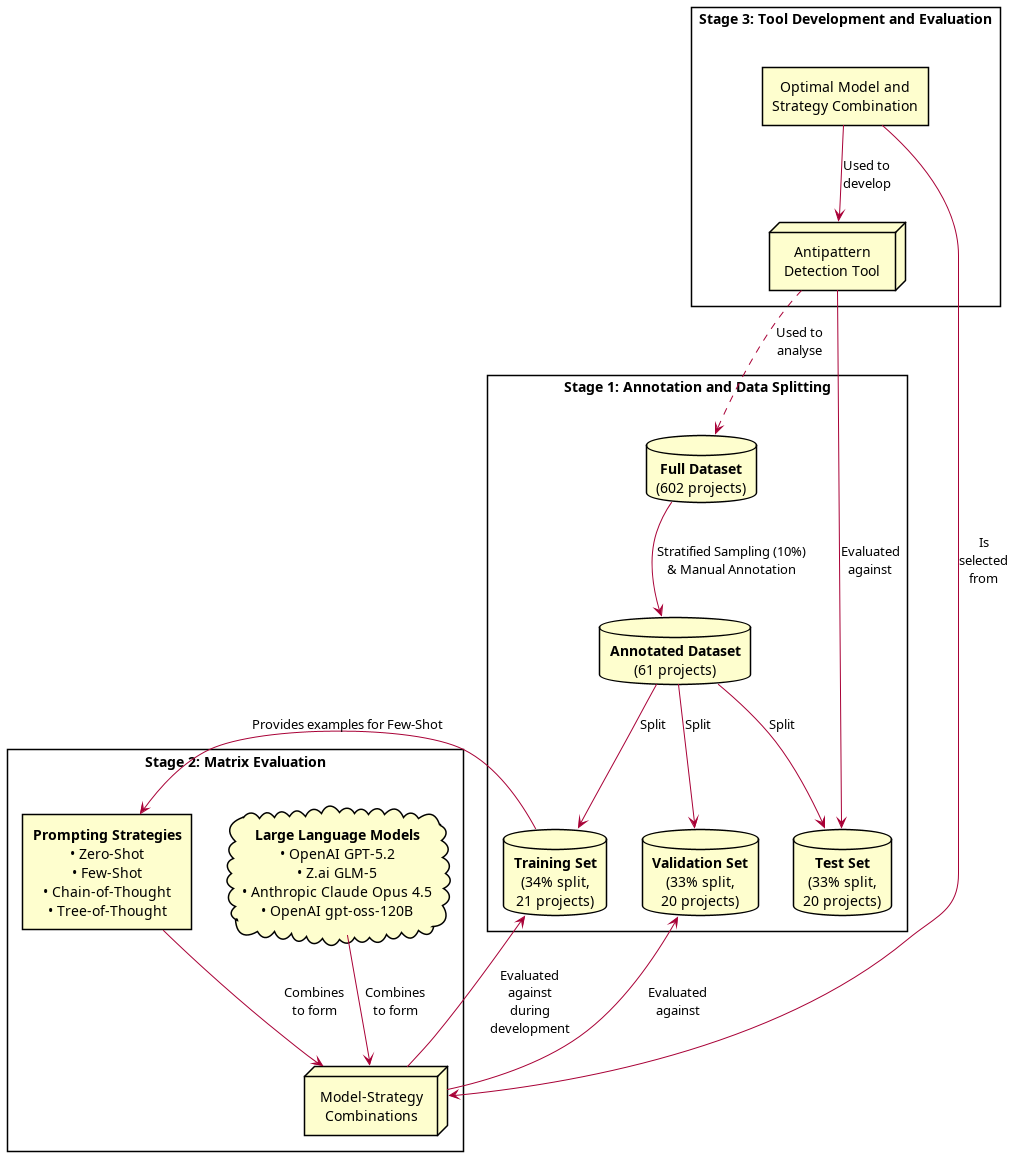
\includegraphics[width=\textwidth]{figures/data_sets_diagram.png}
    \caption{All created datasets with their intended uses.}
    \label{fig:dataSets}
\end{figure}
